À tout moment, vous pouvez changer le mot de passe de votre compte ChromaCase.

Pour changer de mot de passe, rendez-vous sur la page des réglages (Voir Capture \ref{fig:access-settings-password}).

\begin{figure}[H]
	\begin{subfigure}[b]{0.7\textwidth}
		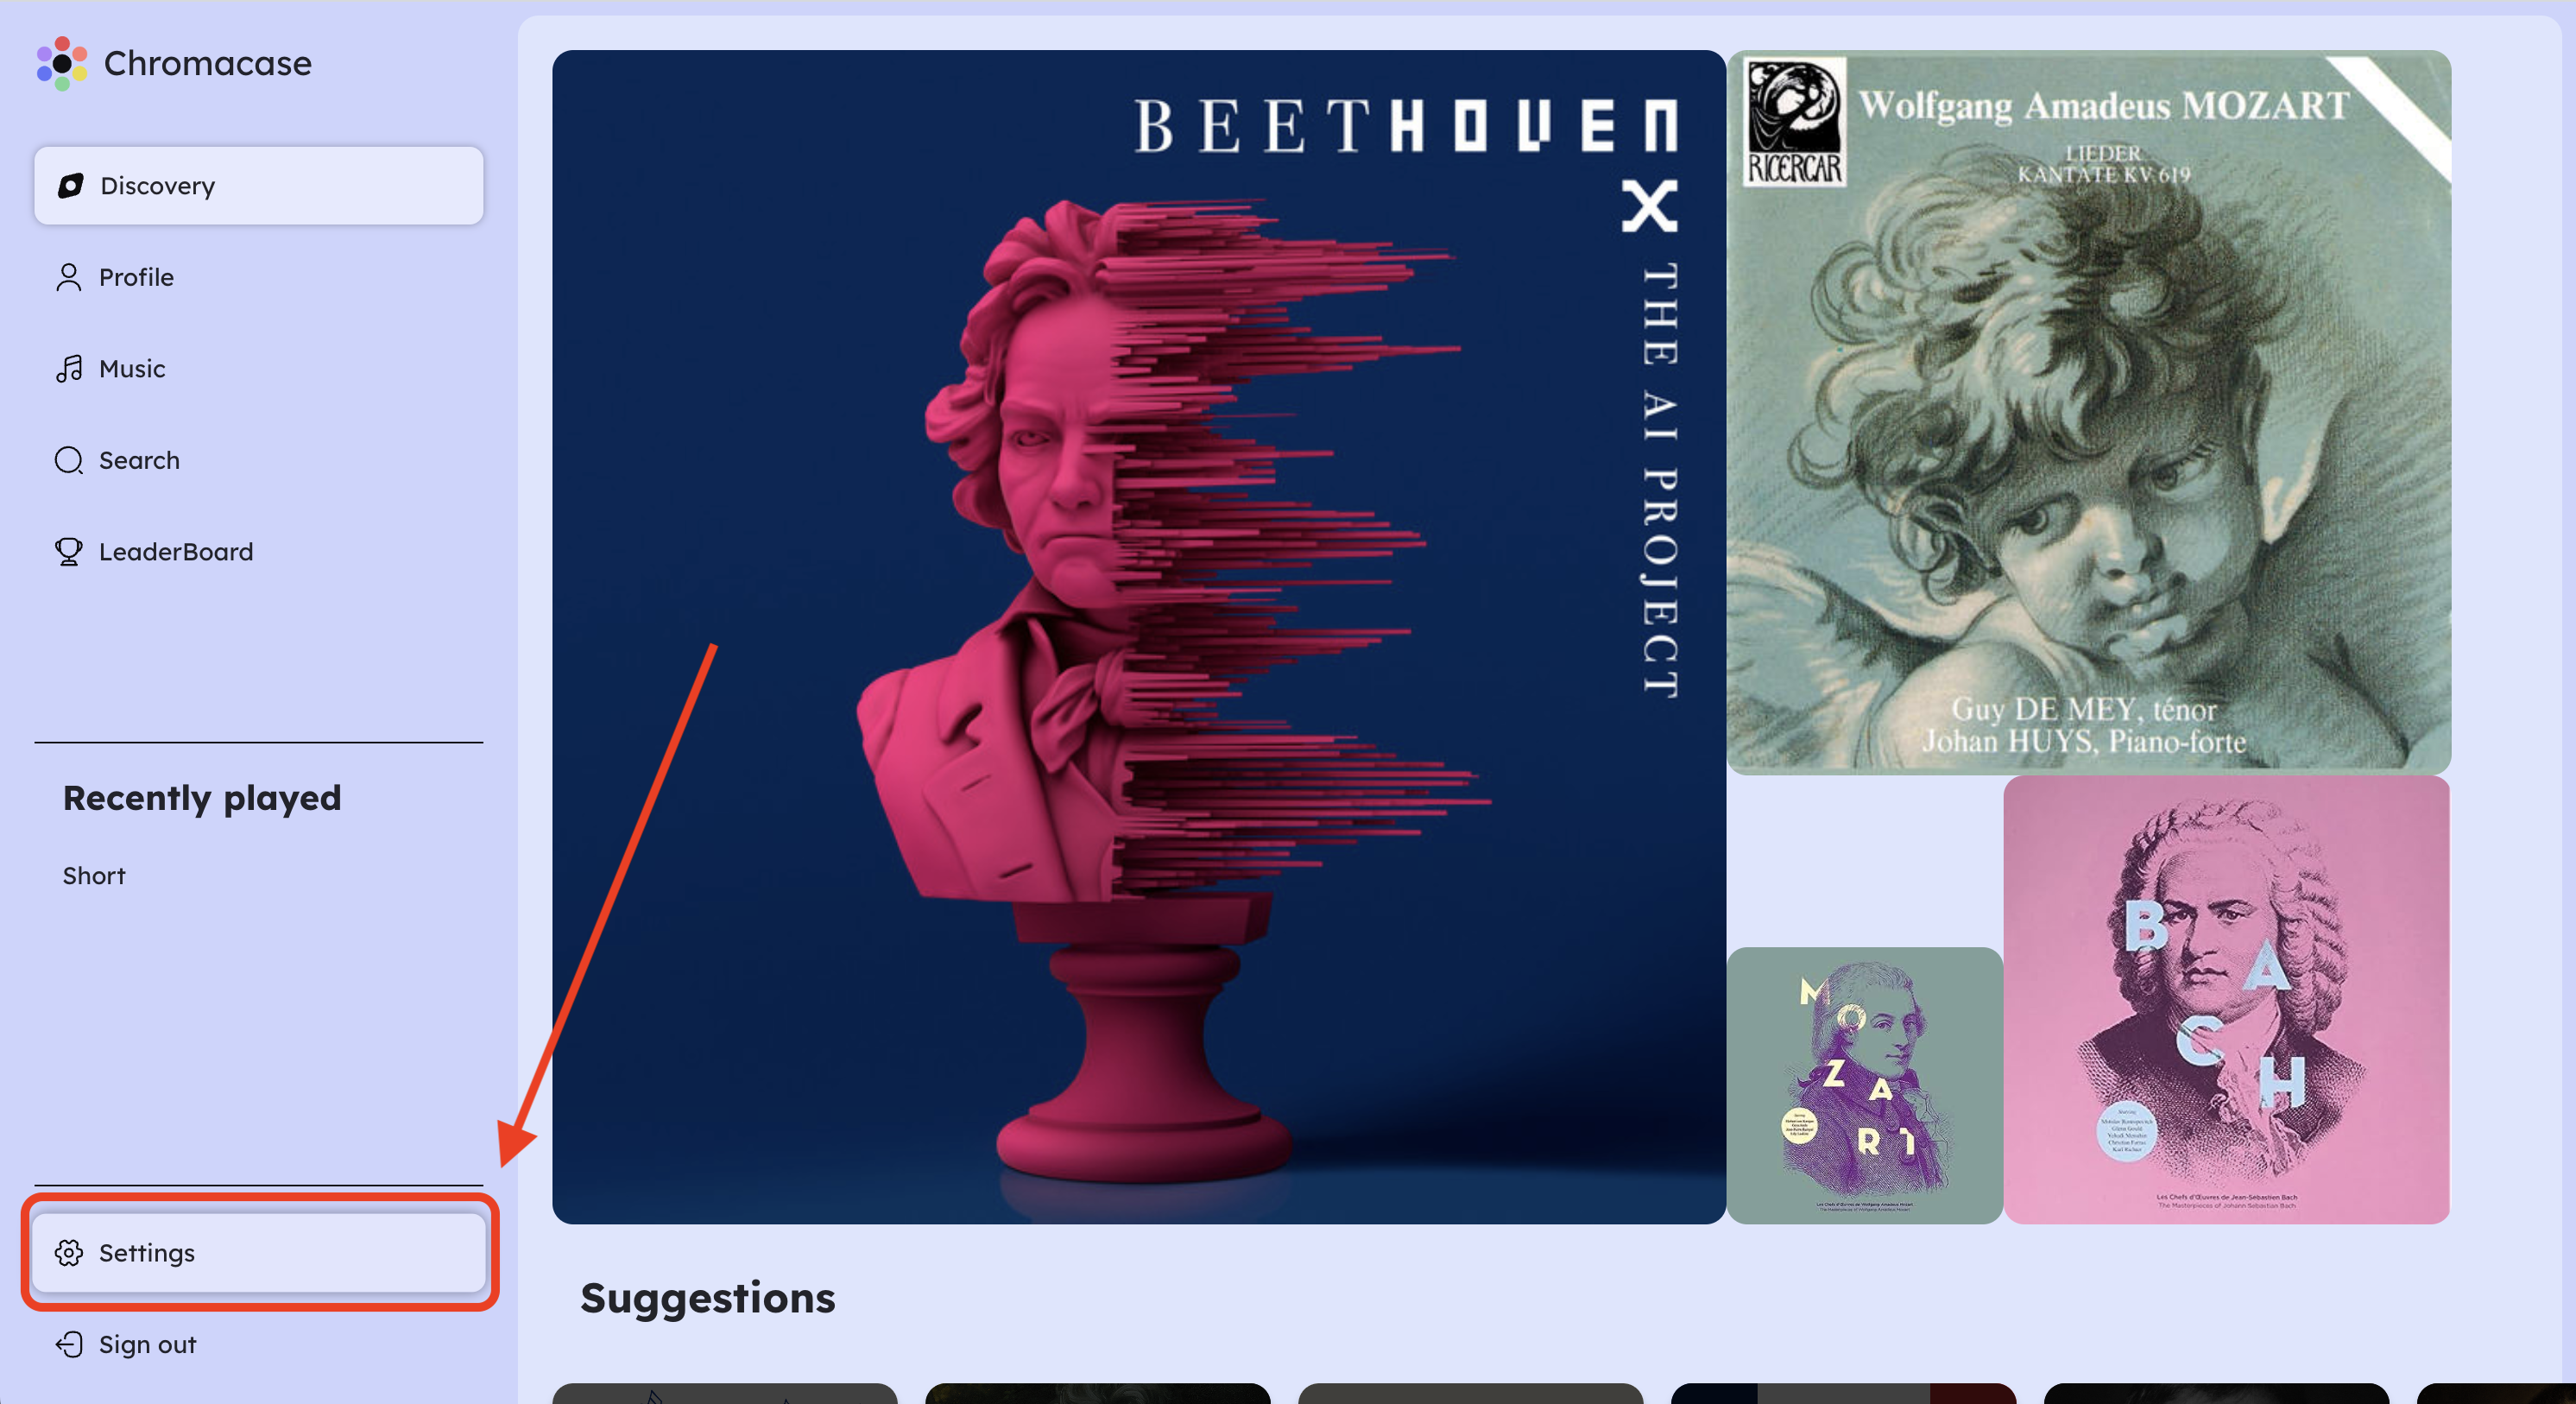
\includegraphics[width=\linewidth]{../\dir/guide/auth/access-settings.png}
		\caption{Version navigateur}
	\end{subfigure}
	\begin{subfigure}[b]{0.25\textwidth}
		
\includegraphics[width=\linewidth]{../\dir/guide/auth/access-settings-mobile.png}
		\caption{Version mobile}
	\end{subfigure}
	\caption{Accéder aux réglages}
	\label{fig:access-settings-password}
\end{figure}

Cliquez sur l'onglet "Profile", puis "Changer le mot de passe", saisissez votre ancien et nouveau mot de passe dans les champs correspondant. Une fois le formulaire rempli, cliquez sur le bouton de validation (Voir Capture \ref{fig:change-password}).

\begin{figure}[H]
	\begin{subfigure}[b]{0.7\textwidth}
		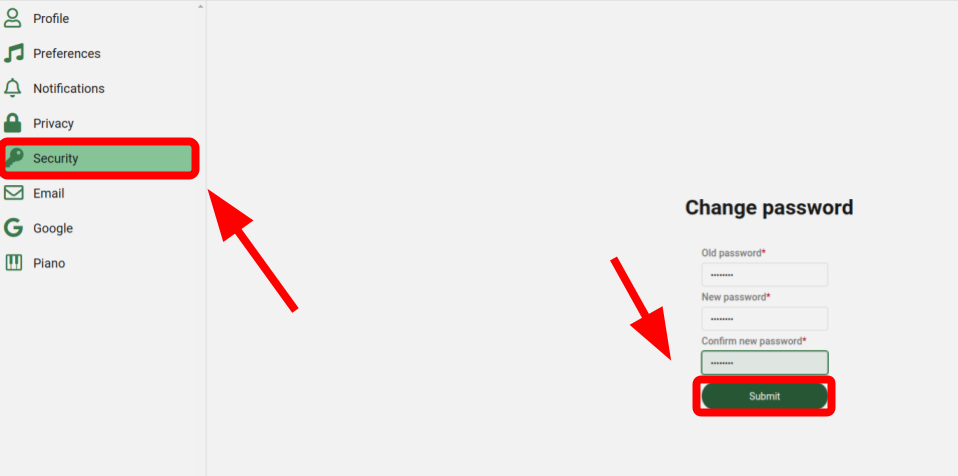
\includegraphics[width=\linewidth]{../\dir/guide/auth/change-password.png}
		\caption{Version navigateur}
	\end{subfigure}
	\begin{subfigure}[b]{0.25\textwidth}
		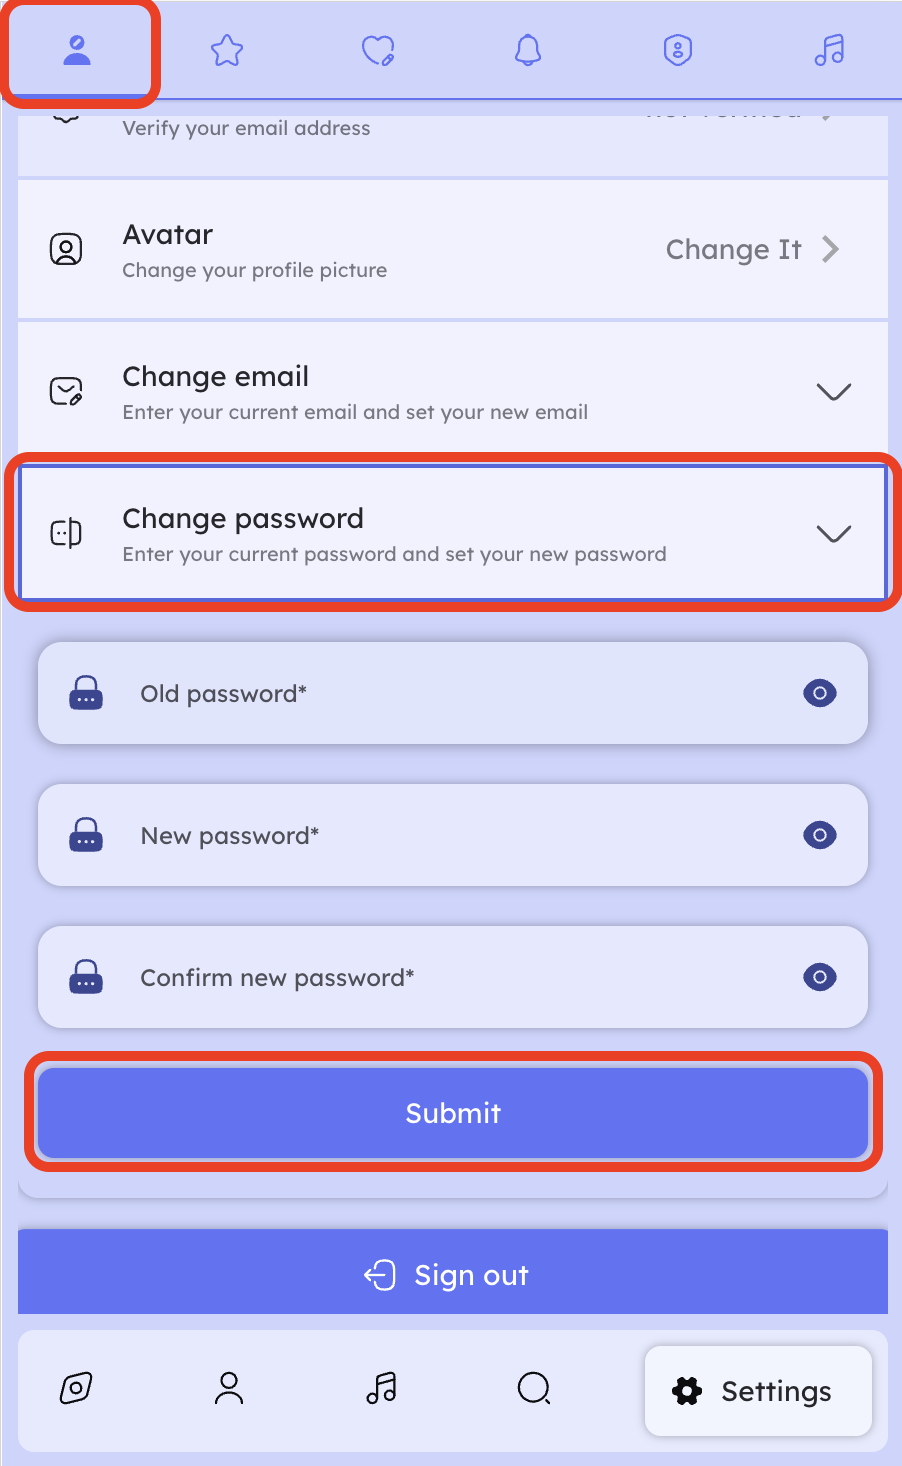
\includegraphics[width=\linewidth]{../\dir/guide/auth/change-password-mobile.png}
		\caption{Version mobile}
	\end{subfigure}
	\caption{Changer de mot de passe}
	\label{fig:change-password}
\end{figure}